\documentclass[a4paper,ngerman,12pt]{exam}
\usepackage{babel}
\usepackage[utf8]{inputenc}
\usepackage[T1]{fontenc}
\usepackage{graphicx}
\usepackage{algpseudocode}
\usepackage{geometry}
\usepackage{csquotes} % Anführungszeichen
\usepackage{paralist} % kompakte Aufzählungen
\usepackage{textcomp,tikz} %diverses
\usepackage{amsmath,amssymb,amstext,amsthm}
\usepackage{listings}
\usepackage{mathtools}
\usepackage{mdframed} % Boxen
\usepackage{float}
\usepackage{tikz}
\usetikzlibrary{calc}
\usetikzlibrary{arrows, automata}

\geometry{a4paper, top=3cm, left=2.7cm, right=2.7cm}
\pagestyle{plain}
\renewcommand{\solutiontitle}{\noindent\textbf{Lösung:}\enspace}
\DeclarePairedDelimiter\ceil{\lceil}{\rceil}
\DeclarePairedDelimiter\floor{\lfloor}{\rfloor}

%\printanswers

\begin{document}
\noindent Theoretische Informatik \hfill Gruppe 8 \\
\mbox{}\hfill Loris Reiff
\begin{center}
  \bfseries\Large
  Quiz 4\ifprintanswers
  -- Lösungen
\fi
\end{center}


\begin{questions}
  \question
Entwerfe einen nichtdeterministischen endlichen Automaten für die Sprache
  \begin{align*}
    L &= \{x \in \{0,1\}^* \mid (x = 01y10 \text{ für } y \in \{0,1\}^+) \text{ oder } |x|=3 \}
  \end{align*}
  \vspace{-1em}
    \begin{solutionorbox}[17em]
\begin{figure}[H]
  \centering
  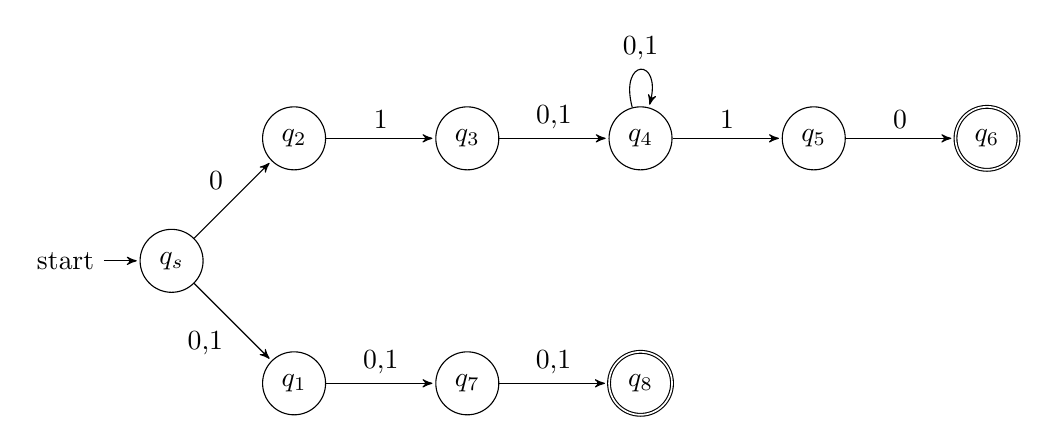
\begin{tikzpicture}[>=stealth', shorten >=1pt, auto, node distance=2.2cm, scale=1, transform shape, align=center, state/.style={circle, draw,minimum size=0.8cm}]
  \node[initial, state]   (q0)                          {$q_s$};
  \node[state]            (q7)     [below right of=q0]  {$q_1$};
  \node[state]            (q3)     [above right of=q0]  {$q_2$};
  \node[state]            (q4)     [right of=q3]        {$q_3$};
  \node[state]            (q5)     [right of=q4]        {$q_4$};
  \node[state]            (q1)     [right of=q5]        {$q_5$};
  \node[state,accepting]  (q6)     [right of=q1]        {$q_6$};
  \node[state]            (q8)     [right of=q7]        {$q_7$};
  \node[state,accepting]  (q9)     [right of=q8]        {$q_8$};

  \path[->]
        (q0)        edge                node [above left] {0} (q3)
                    edge                node [below left] {0,1} (q7)
        (q3)        edge                node [above] {1} (q4)
        (q4)        edge                node [above] {0,1} (q5)
        (q5)        edge                node [above] {1} (q1)
                    edge [loop above]   node [above] {0,1} (q5)
        (q7)        edge                node [above] {0,1} (q8)
        (q8)        edge                node [above] {0,1} (q9)
        (q1)        edge                node [above] {0} (q6)
        ;

\end{tikzpicture}
\end{figure}
    \end{solutionorbox}

\question
Verwende die Potenzmengenkonstruktion, um den folgenden nichtdeterministischen endlichen Automaten in einen
äquivalenten deterministischen Automaten umzuwandeln.\\
\textit{Nicht erreichbare Zustände weglassen}
\begin{figure}[H]
  \centering
  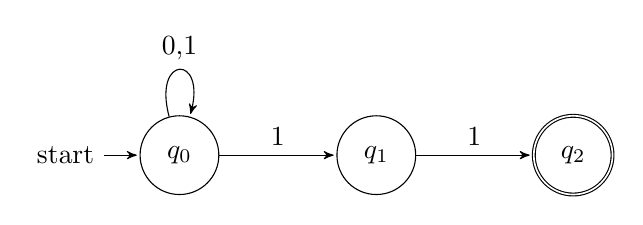
\begin{tikzpicture}[>=stealth', shorten >=1pt, auto, node distance=2.5cm, scale=1, transform shape, align=center, state/.style={circle, draw,minimum size=1cm}]
  \node[initial, state]   (q0)                    {$q_0$};
  \node[state]            (q1)     [right of=q0]  {$q_1$};
  \node[state,accepting]   (q2)     [right of=q1]  {$q_2$};

  \path[->]
        (q0) edge                node [above] {1}   (q1)
             edge [loop above]   node [above] {0,1} (q0)
        (q1) edge                node [above] {1}   (q2)
        ;
\end{tikzpicture}
\end{figure}
  \vspace{-1em}
    \begin{solutionorbox}[17em]
\begin{figure}[H]
  \centering
  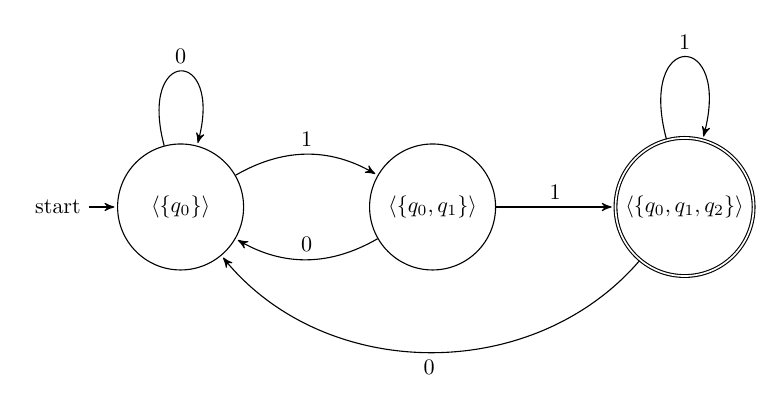
\begin{tikzpicture}[>=stealth', shorten >=1pt, auto, node distance=4cm, scale=0.8, transform shape, align=center, state/.style={circle, draw,minimum size=2cm}]
    \node[initial, state]  (q0)                    {$\langle \{q_0\} \rangle$};
    \node[state]           (q1)     [right of=q0]  {$\langle \{q_0, q_1\}\rangle$};
    \node[state,accepting]   (q2)     [right of=q1]  {$\langle \{q_0, q_1, q_2\}\rangle$};

  \path[->]
        (q0) edge [bend left]    node [above] {1}   (q1)
             edge [loop above]   node [above] {0}   (q0)
        (q1) edge                node [above] {1}   (q2)
             edge [bend left]    node [above] {0}   (q0)
        (q2) edge [loop above]   node [above] {1}   (q2)
             edge [bend left=50]    node [below] {0}   (q0)
        ;
\end{tikzpicture}
\end{figure}
    \end{solutionorbox}

\question
Zeige dass
\begin{align*}
  \{w \in \{a,b\}^* \mid |w|_a = |w|_b\} \not\in \mathcal{L}_{\mathrm{EA}}
\end{align*}
\textit{(Aufgabe 3.14 (a) aus dem Buch)}
    \begin{solutionorbox}[20em]
    Sei $A = (Q, \{a, b\}, \hat{\delta}_A, q_0, F)$ ein EA mit $L(A) = L$.
    Beachten wir die Wörter
    \begin{align*}
      a, aa, \dots , a^{|Q|+1}
    \end{align*}
    Es existieren also $i, j \in \{1, 2, \dots, |Q|+1\}$ mit $i < j$
    und
    \begin{align*}
      \hat{\delta}_A(q_0, a^i) &= \hat{\delta}_A(q_0, a^j)
    \end{align*}
    (Schubfachprinzip)\\
    Gemäss Lemma 3.3 im Buch gilt somit
    \begin{align*}
      a^i z \in L &\iff a^j z \in L
    \end{align*}
    für alle $z \in \{a, b\}^*$. Für $z = b^i$ haben wir aber einen Widerspruch:
    $a^i b^i \in L$ und $a^j b^i \not\in L$. Das heisst also, dass
    es keinen EA für L gibt.
    \end{solutionorbox}
\end{questions}

\end{document}
